% Author Vahid Partovi Nia
% Copyright Huawei Technologies
% Network Mind Team



\documentclass[12pt]{beamer}

\usetheme{Hannover}
\setbeamercolor{section in sidebar shaded}{fg=black}

\usecolortheme{beaver}
\beamertemplatenavigationsymbolsempty

%  \usebeamertemplate{navigation symbols}\hfill
%  \insertframenumber{}/\inserttotalframenumber}
  

\useoutertheme{sidebar}
\pgfdeclareimage[width=2.5\baselineskip]{institut-logo}{fig/mcgill_logo}
\setbeamertemplate{footline}
{\raisebox{-2ex}{\pgfuseimage{institut-logo}}
%  \hfill
\hspace{5cm}
  \usebeamertemplate{navigation symbols}
  \insertframenumber{}/\inserttotalframenumber
  \hspace{3.8cm}
YCBS255
}
%\setbeamertemplate{sidebar right}{}
  
\setbeamercolor{block title}{fg=darkred}
\setbeamercolor{local structure}{fg=darkred}

\setbeamercolor{palette sidebar secondary}{fg=darkgray, bg=white}



\usefonttheme{professionalfonts} % using non standard fonts for beamer


\makeatletter
\beamer@nav@subsectionstyle{hide/hide/hide}
\makeatother

\titlegraphic{\includegraphics[width=2cm]{fig/mcgill_logo}}





\def \y {\mathbf y}
\def \X {\mathbf X}
\def \A {\mathbf A}
\def \t {^\top}
\def \inv {^ {-1}}
\def \x {\mathbf x}
\def \z {\mathbf z}
\def \bbeta {\boldsymbol \beta}
\def \eeps {\boldsymbol \varepsilon}
\def \OOmega {\boldsymbol \Omega}

\def \ttheta {\boldsymbol \theta}

\def \Q {\mathbf Q}
\def \R {\mathbf R}
\def \q {\mathbf q}
\def \zero {\mathbf 0}

\def \r {\mathbf r}

\def \L {\mathbf L}
\def \U {\mathbf U}
\def \real {{\rm I\!R}}
\def \A {\mathbf A}
\def \P {\mathbf P}

\def \D {\mathbf D}
\def \MSE {\mathrm{MSE}}
\def \E {\mathbb{E}}
\def \V {\mathbb{V}}
\def \KL {\mathbb{KL}}
\def \H {\mathbb{H}}

\def \sumi {\sum_{i=1}^n}
\def \sumj {\sum_{j=1}^p}

\def \argmin {\mathrm {argmin}~}
\def \argmax {\mathrm {argmax}~}
\def \tr {\mathrm {tr}}
\def \sign {\mathrm {sign}}
\def \N {\mathcal{N}}
\def \eye {\mathbf{I}}
\def \I {\mathbf{I}}
\def \ind {\mathbb{I}}

\begin{document}

% no title and no author on sidebar
\title[]{Cross-validation and Splines}   
\author[]{Vahid Partovi Nia} 
\institute{Advanced Machine Learning: Lecture 05}
\date{\today} 


\makeatletter
  \begin{frame}[plain]
    \hspace*{-\beamer@leftsidebar}%
    \advance\textwidth by \beamer@leftsidebar\relax
    \beamer@leftsidebar=\z@
    \begin{minipage}{\textwidth}\par%
      \maketitle
    \end{minipage}
  \end{frame}
  \makeatother



\frame{\frametitle{Outline}\tableofcontents} 

\setbeamertemplate{sidebar left}[sidebar theme]

\section{Splines}

\frame{\frametitle{univariate function approximation}
Suppose approximation of a good univariate function over a set of observed $(x_i, y_i), i=1,\ldots, n.$
$$y_i =f(x_i)+\varepsilon_i \approx \sum_{j} \beta_j b_j(x_i)$$
\begin{itemize}
\item polynomial base $x \in [-1,1]$,  $b_j(x_i) = x_i ^j$ 
\item Fourier base $x\in[-\pi, \pi]$,  $$y_i \approx \sum_{j=1}^k \beta^{(1)}_j \sin\left({2\pi j \over k} \right)  + \beta^{(2)}_j\cos \left({2\pi j \over k} \right) $$
\item Wavelet base of resolution $k$, $x \in [0,2\pi]$ 
$$y_i \approx \sum_{j=1}^{2^k -1 } \beta^{(k)}_j b^{(k)}_j(x_i) $$
\end{itemize}
}


\frame{\frametitle{Piecewise polynomials}
\includegraphics[width=0.4\textwidth]{fig/fig5-1-01}
\includegraphics[width=0.4\textwidth]{fig/fig5-1-02}\\
\includegraphics[width=0.4\textwidth]{fig/fig5-1-03}
}

\frame{\frametitle{Cubic}
\includegraphics[width=0.4\textwidth]{fig/fig5-2-01}
\includegraphics[width=0.4\textwidth]{fig/fig5-2-02}\\
\includegraphics[width=0.4\textwidth]{fig/fig5-2-03}
\includegraphics[width=0.4\textwidth]{fig/fig5-2-04}
}

\frame{\frametitle{Cubic}
\includegraphics[width=0.4\textwidth]{fig/fig5-1-04}\\
Multivariate $=$ Additive Model
$$y_i \approx f(\x_i) = \sum_{j=1}^p f_j(x_{ij})$$
}



\frame{\frametitle{B-Spline}
B splines of order $m$ are piece-wise polynomial functions
\begin{eqnarray*}
h_j(x) &=& x^j, j=0,\ldots,m \\
h_{m+l}(x) &=& \{\max(0, x-\xi_l)\}^{m-1}
\end{eqnarray*}
}

\frame{\frametitle{Bsplines}
\begin{itemize}
\item Bsplines of order $m>1$ are continuous
\item They have continuous derivative up to $m-2$
\item Cubic splines are Bsplines of order $m=4$
\item Natural splines, are cubic splines with $x_i = \xi_i$
\item Smoothing splines are natural splines are generalized ridge with penalization $\bbeta\t\OOmega\bbeta$
\item $\OOmega=  [\omega_{l,k}]$ is not a diagonal matrix.
\item $\omega_{l,k} = \int h''_{m+l}(x) h''_{m+k}(x)dx$
\end{itemize}
}

\frame{\frametitle{Reproducing Kernel Hilbert Space}
\begin{itemize}
\item Suppose $$\hat f = \argmin \sum_{i=1}^n L(y_i, f(x_i) ) + \lambda || f || $$
\item Many function estimation problems fall in this context, like splines, support vector machines, kernel smoothers, local regression, etc.
\item Suppose a positive definite kernel function $K(x,x')$ defines the space of the Hilbert space. 
\item Take some arbitrary values of $x_j \in \real$ and generate a function $f(x) = \sum_j \beta_j K(x,x_j) \in \mathcal H_K$
\end{itemize}
}
\frame{\frametitle{Kernel}
\begin{itemize}
\item Suppose $K(x,x')= \sum_{j=1}^\infty \gamma_j \phi_j(x)\phi_j(x')$  with $\gamma_j >0, \sum_j \gamma_j^2<\infty$
\item Then all function in $\mathcal H_K$ have an eigen expansion $f(x)= \sum_{j=1}^\infty c_j \phi_j(x)$
\item Define $|| f || = \sum_{j=1}^\infty c_j^2 / \gamma_j$
\end{itemize}
}
\frame{\frametitle{Solution}
Solution to 
\begin{eqnarray*}
\hat f(x) &=&  \argmin L(y_i, f(x_i) ) + \lambda || f || \\
&=& \argmin   \sum_{i=1}^n L\left( y_i, \sum_{j=1}^\infty c_j \phi_j(x_i) \right) +\lambda \sum_{j=1}^\infty c_j^2/\gamma_j 
\end{eqnarray*}
has a finite dimensional solution
$$\hat f(x) = \sum_{i=1}^n \beta_i K(x,x_i) $$ 
and 
$$|| f || = \sum_{i=1}^n \sum_{i'=1}^n K(x_i, x_{i'}) \beta_i \beta_i' $$

}
\frame{\frametitle{Generalized ridge}
\begin{eqnarray*}
\hat \bbeta &=&   \argmin (\y - \mathbf K\bbeta )\t (\y - \mathbf K\bbeta ) + \lambda \bbeta\t \mathbf K \bbeta  \\
\hat f(x) &=& \mathbf K\hat \bbeta 
\end{eqnarray*}
Take $L(y_i , f(x_i)) = \max(0, 1-y_i f(x_i))$ to produce support vector machines.
}
\section{Kernel smoothing}
\frame{
\centering
Kernel Smoothing
}
\frame{\frametitle{}
\includegraphics[width=0.8\textwidth]{fig/smooth00}
}


\frame{\frametitle{}
\includegraphics[width=0.8\textwidth]{fig/smooth01}
}

\frame{\frametitle{}
\includegraphics[width=0.8\textwidth]{fig/smooth02}
}

\frame{\frametitle{}
\includegraphics[width=0.8\textwidth]{fig/smooth03}
}

\frame{\frametitle{}
\includegraphics[width=0.8\textwidth]{fig/smooth00}
}

\frame{\frametitle{}
\includegraphics[width=0.8\textwidth]{fig/smooth05}
}

\frame{\frametitle{}
\includegraphics[width=0.8\textwidth]{fig/smooth06}
}

\frame{\frametitle{}
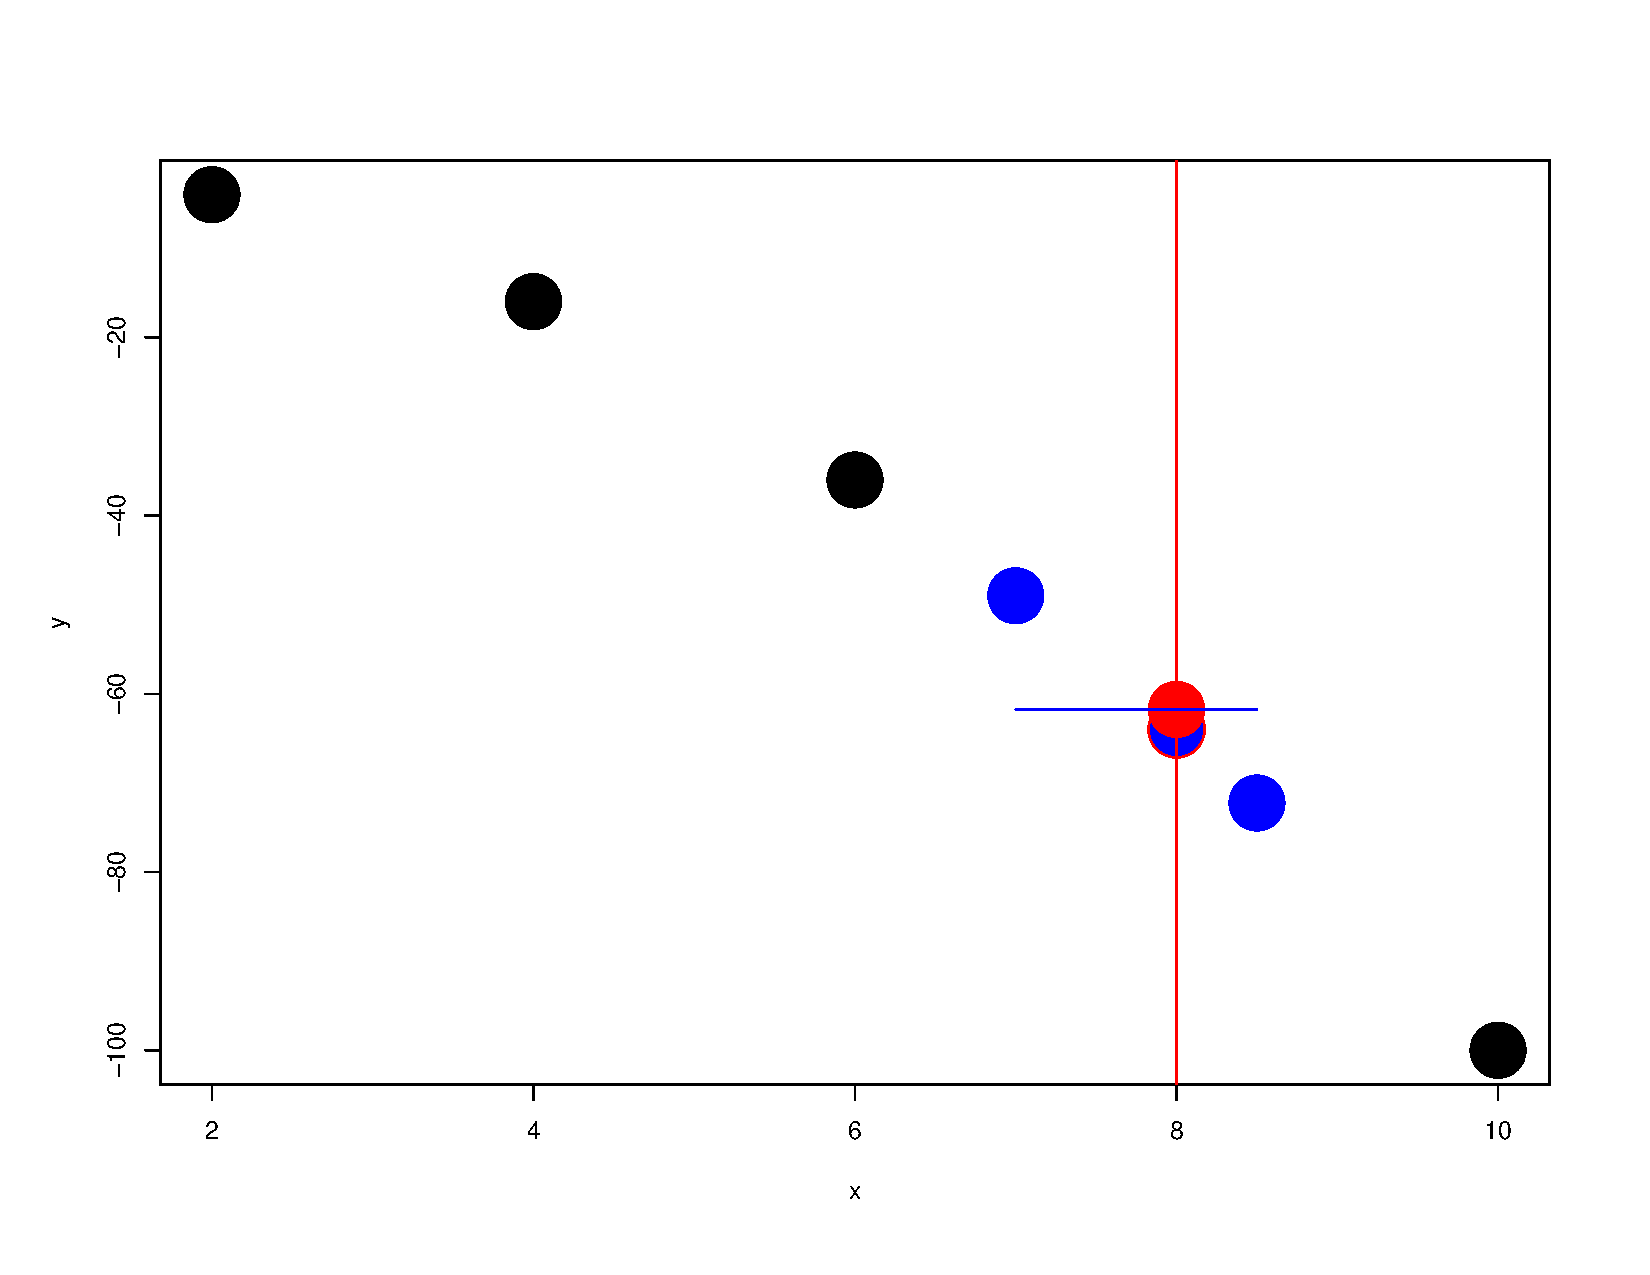
\includegraphics[width=0.8\textwidth]{fig/smooth07}
}


\frame{\frametitle{non-parametric function}
\begin{itemize}
\item Define a neighbourhood of $x$
\item $\hat f(x_0) ={1\over || N(x_0) || } \sum\limits_{i\in N(x_0)} y_i $
\item  $w_i(x_0)=\ind_{A}(x_0), A=\{x\in\real , || x_0 - x_i || < \lambda \}$
$$ \hat f(x_0) = {\sum_{i=1}^n w_i(x_0) y_i \over \sum_{i=1}^n w_i(x_0)}$$
\item $w_i(x_0) = K(x_0, x_i)$
\item $$ \hat \beta_0(x_0)  = \argmin \sum_{i=1}^n K(x_0,x_i)(y_i - \beta_0)^2 $$
\end{itemize}

}



\frame{\frametitle{Uniform Kernel}
\includegraphics[width=0.5\textwidth]{fig/fig6-1-01}
}

\frame{\frametitle{Smooth Kernel}
\includegraphics[width=0.5\textwidth]{fig/fig6-1-02}
}


\frame{\frametitle{Constant versus linear}
\includegraphics[width=0.3\textwidth]{fig/fig6-3-01} ~~
\includegraphics[width=0.3\textwidth]{fig/fig6-3-02}
}

\frame{\frametitle{transformed kernel}
\includegraphics[width=0.3\textwidth]{fig/fig6-4-01} ~~
\includegraphics[width=0.3\textwidth]{fig/fig6-4-02}
}

\frame{\frametitle{Kernel functions}
\includegraphics[width=0.8\textwidth]{fig/kernels}
}
\frame{\frametitle{Smooth histograms}
\includegraphics[width=0.8\textwidth]{fig/histsmooth}
}
%\frame{\frametitle{}
%\includegraphics[width=0.8\textwidth]{fig/}
%}






\end{document}
